
\section{Lecture 33: Ideal gas law}

While liquids are almost entirely incompressible, as we have seen, gases are not. In a liquid, the molecules are still moving around (as opposed to a solid), but are quite closely packed, at least compared to a gas. In a gas, there is a fairly large distances between molecules, unless the pressure is very high. Therefore, we can compress gases rather easily, until the molecules become about as closely packed as in a liquid. If we keep compressing a gas at that point, it may undergo a phase change, usually to a liquid, but this depends on the compound. Carbon dioxide is perhaps the most well-known compound to only exist in gas and solid phases at atmospheric pressures; the liquid phase only exists at higher pressures (higher than about 5.1 atmospheres), so it either \emph{deposits} (goes from gas directly to solid) or \emph{sublimes} (also known as sublimates), meaning it goes from solid directly to gas.\\
Air at 1 atmosphere has a density 1/1000 times that of water; that says something about the relative distances between molecules involved.

Here are some definitions we'll soon use, from a lecture supplement sheet:

\begin{center}
\begin{tabular}{|r|l|l|}
\hline
Symbol & Meaning & Unit/value\\ \hline
P & Pressure & Pascal ($\text{N/m}^2$)\\
V & Volume & $\text{m}^3$\\
T & Temperature & Kelvin (K)\\
N & Number of molecules & \\
n & Number of moles (see below) & mol\\
$\text{N}_\text{A}$ & Avogadro's constant & $6.022 \times 10^{23} \text{mol}^{-1}$ \\
R & Universal gas constant & \SI{8.31}{J/(K mol)}\\
k & Boltzmann constant & $R/N_A = \SI{1.38e-23}{J/K}$\\
Z & number of protons in a nucleus & \\
N &  number of neutrons in a nucleus & \\
A & atomic number, $A = Z + N$ & \\ \hline
\end{tabular}
\end{center}

We will use the unit of a \emph{mole}, which is a unit not unlike terms like a dozen, only way larger. 1 mol is defined as the number of atoms in 12 grams of carbon-12; 1 mol of water means approximately $6.022 \times 10^{23}$ molecules of water, for example. The unit can be used for anything. 1 mol of eggs is a lot; something like $10^{12}$ eggs were produced in 2002, so 1 mol of eggs would, at that rate, take 602 214 129 000 years to produce! Nevertheless, it is not much more than a number -- only that it has a unit attached to it. I think I'll stick to dozens as far as eggs go.

Note that moles are about a number of something, but not \emph{necessarily} number of \emph{atoms}. One mole of helium molecules is the same as one mole of helium atoms, since helium doesn't tend to group into molecules at all.\\
On the other hand, one mole of oxygen gas ($O_2$) contains 2 moles of oxygen atoms. Unless specified otherwise, one mole will here refer to the molecular count, so that 1 mole of carbon dioxide and 1 mole of helium has the same number of molecules, but \emph{not} the same number of individual atoms.

\subsection{Ideal gas law}

The \emph{ideal gas law} states that

\begin{equation}
P V = n R T
\end{equation}

using the definitions we introduced above. Both sides of this equation have the dimension of energy, i.e. units of joules using the MKS units. $P V$ has units of $(\text{N/m}^2)(\text{m}^3) = \text{N m} = \text{J}$, while $n R T$ has units of $(\text{mol})(\text{J/(K mol)})(\text{K}) = \text{J}$.

Using the Boltzmann constant $k = R/N_A \approx \SI{1.38e-23}{J/K}$ that we listed in the table above, we can also write the ideal gas law as

\begin{equation}
P V = N k T
\end{equation}

where $N$ is now a dimensionless number relating the number of molecules (not in moles, but the actual number), $k$ is the Boltzmann constant as in the table above, and the rest of the variables remain as they were.

Before we use the ideal gas law, we'll have a quick look at atomic number and related things.\\
An atom has $Z$ protons (that define which element it is), $N$ neutrons (which define the isotope) and, if it is electrically neutral (i.e. not an ion), also $Z$ electrons to balance out the change. (As we learn in 8.02 if not in high school, the proton and the electron have exactly the same magnitude of change, only opposite signs.)\\
The \emph{atomic mass number} $A$ is then simply $A = Z + N$, and defines how many protons plus neutrons there are in the nucleus.\\
Protons and neutrons have very close to the same mass (they differ by about 0.14\%), while is this context, electrons have almost zero mass (an electron only has 0.05\% of a proton's mass) that we can often neglect.

Let's look at carbon as an example. Carbon has 6 protons (6 protons defines the element, so anything else wouldn't be carbon). Carbon-12 also has 6 neutrons, so $A = 12$, which is also what we specify in its name.\\
Other forms of carbon have differing number of neutrons; known isotopes range from carbon-8 (2 neutrons) to carbon-22 (16 neutrons), though most of these are highly unstable. Only carbon-12 and carbon-13 are stable; carbon-14 has a half-life of 5730 years and is commonly used for radiometric dating of organic things.

As shown in the definition above, 1 mol of carbon-12 has a mass of 12 grams exactly. 1 mol of carbon-14 has a mass of approximately 14 grams (the approximate mass of 1 mol, in grams, of any atom is simply the number of nucleons), though because of the small difference in mass between protons and neutrons, the actual mass is closer to 14.00324 g.

Another example would be that of oxygen gas; it has a \emph{molar mass} of about 32 g/mol. Each oxygen atom has 8 protons and 8 neutrons (some oxygen atoms are oxygen-17 and oxygen-18, but the vast majority are oxygen-16, so the average atomic mass number is about 16). Each $O_2$ molecule consists of two oxygen atoms, so we find $2 \times (8 + 8) = 32$ g/mol.

Since the mass of a proton and a neutron is almost equal, we can to a reasonable approximation write the mass of a molecule as $m_{molecule} = A \times \SI{1.67e-27}{kg}$, where the mass of a proton is $m_p \approx \SI{1.672621e-27}{kg}$.

\subsection{Ideal gas law example}

The ideal gas law is an approximation, but one that holds reasonably well for most gases. Therefore, we don't need to specify what the gas is to use it.

Say we have a gas at 1 atmosphere, so $P \approx \SI{1.03e5}{Pa}$. We also have $n = \SI{1}{mol}$ of the substance. We do this at room temperature, so $T = \SI{293}{K}$.

$P V = n R T$, and we know everything except $V$. ($R$ is a constant, so we know that, too.)\\
We solve for $V$, and find

\begin{equation}
V = \frac{n R T}{P} = \frac{(\SI{1}{mol})(\SI{8.31}{J/(K mol)})(\SI{293}{K})}{\SI{1.03e5}{Pa}} \approx \SI{0.0236}{m^3} \approx \SI{23.6}{L}
\end{equation}

So this is (approximately) true whether the gas is helium, oxygen, nitrogen etc., as long as there is 1 atm of pressure. Of course, this only holds as long as the substance in question would actually \emph{be} a gas as this temperature and pressure. If we try to use water at 1 atmosphere and room temperature, then our results will be nonsense; we still find almost 24 liters, but the correct answer is about 18 mL, so this ``estimate'' is over 1000 times too high. (It also doesn't hold very well for water vapor either, because water molecules are fairly attracted to each other, which makes the ideal gas law not hold.)\\
We will soon look at phase diagrams, which will help us figure out whether a substance will be a gas, liquid or solid (or a mixture of two or three of these) at a given temperature--pressure combination.

As the name implies, the law is exactly true for \emph{ideal} gases (by definition: an ideal gas is one that obeys this law). Many real gases are close to ideal under common circumstances, though. 1 mole of oxygen at atmospheric pressure and room temperature is within 0.1\% of what the ideal gas law predicts (the true value is smaller than the approximation). At 20 atmospheres, the result is about 2\% off, still with the correct result being smaller than the approximation.

\subsection{Ideal gas law with different molar mass gases}

Consider the case when we have two gases where the molar masses are very different, but we have the same number of moles of each gas. Both are at room temperature, and they are in identical containers. $n$, $T$ and $V$ are the same, and via the ideal as law, that means $P$ is also the same. The masses of the molecules are very different however, and since we have the same amount, the total mass of one gas must also be much greater than the mass of the other.

The molecules in the gas are flying around in all directions, with different speeds. We consider an average speed $\overbar{v}$ for simplicity.\\
Say a molecule of mass $m$ hits the container wall with speed $\overbar{v}$. It bounces back in an elastic collision, which implies a momentum change of $2 m \overbar{v}$ in magnitude -- its forward momentum is replaced with backwards momentum of the same magnitude.

That is just the momentum change of one molecule, though. We want the rate of momentum transfer over time.

If we consider a cube of side $L$, it takes a molecule a time $t = \dfrac{2 L}{v}$ to come back to a wall after bouncing off it, in the simple case where it moves in one dimension only. Therefore, the rate of momentum transfer (per second) is $\dfrac{2 m v}{t} = \dfrac{2 m v}{\frac{2 L}{v}} = \frac{m v^2}{L}$. (Thanks to Grove for this derivation.)

The rate of momentum transfer for the entire system is therefore proportional to $m v^2$. Rate of momentum transfer is force, and force is proportional to pressure. It certainly looks as if $m \propto P$ -- which the ideal gas law clearly says is not the case!\\
The only way this works out, and how it actually does work, is if $m v^2$ is constant for a given temperature, i.e. it is independent of $m$! In other words, the speed of the particle is such that it balances out its mass; the smaller the mass, the larger the speed, and vice versa.

For example, comparing helium and oxygen gas, we can write that

\begin{equation}
m_{He} \overbar{v_{He}}^2 = m_{O_2} \overbar{v_{O_2}}^2
\end{equation}
\begin{equation}
\overbar{v_{He}} = \sqrt{\frac{m_{O_2}}{m_{He}}}\ \overbar{v_{O_2}}
\end{equation}

Oxygen molecules have an average speed of about 480 m/s at room temperature. Since the ratio of masses here is about 8, helium molecules move, on average, about $\sqrt{8} \approx 2.82$ times faster than oxygen molecules, which is about 1350 m/s.\\
If we mix the two cases, the only way the ideal gas law can hold is if these speeds still stay true, so that the lighter molecules move faster.

\subsection{Ideal gas law example \#2}

``A closed container with a volume of $\SI{8000}{cm^3}$ is filled with Xenon gas. The gas temperature is 273 K (the container is placed in ice water) and the pressure is 2.0 atm.

How many moles of Xenon are in the container?''

Well, we use $P V = n R T$. We want $n$, so

\begin{equation}
n = \frac{PV}{RT} = \frac{(2\times\SI{1.03e5}{Pa})(\SI{0.008}{m^3})}{(\SI{8.31}{J/(K mol)})(\SI{273}{K})} \approx \SI{0.726}{mol}
\end{equation}

``The container is now submerged in boiling water until the gas inside the container is at 373 K. You may assume that the increase in volume of the container is negligible.

What is the pressure of the xenon?''

We re-rearrange the equation to give
\begin{equation}
P = \frac{n R T}{V}
\end{equation}

Plugging in the given numbers, plus the $n$ we found above,

\begin{equation}
P = \frac{n R T}{V} = \frac{ (\SI{0.726}{mol})(\SI{8.31}{J/(K mol)})(\SI{373}{K})}{\SI{0.008}{m^3}} \approx \SI{281300}{Pa} = \SI{2.7}{atm}
\end{equation}

\subsection{Phase diagrams}

We will now look at phase diagrams. The \emph{phase} of a substance is basically whether it is a solid, liquid or a gas; however, phase and state of matter are not the same thing. For example, while all water ice is solid (its state of matter), there are many different phases. Ice Ih is by far the most common water ice; Ice Ic essentially the only other form naturally occurring on Earth. Over a dozen other forms of water ice have been created in labs, by varying the temperatures and pressures.\\
I will mostly (perhaps entirely) use phase and state of matter interchangeably in the rest of these notes.

Here's a simple, general phase diagram:

\begin{figure}[H]
  \centering
\begin{tikzpicture}[scale=0.4]
  \message{Phase diagrams^^J}
  
  \def\xtick#1#2{\draw[thick] (#1)++(0,.2) --++ (0,-.4) node[below=-.5pt,scale=0.7] {#2};}
  \def\ytick#1#2{\draw[thick] (#1)++(.2,0) --++ (-.4,0) node[left=-.5pt,scale=0.7] {#2};}
  
  % COORDINATES
  \coordinate (O) at (0,0);
  \coordinate (N1) at (2,10);
  \coordinate (N2) at (11,10);
  \coordinate (NE) at (12,10);
  \coordinate (NW) at (0,10);
  \coordinate (SE) at (12,0);
  \coordinate (W) at (0,5);
  \coordinate (S) at (6,0);
  \coordinate (C) at (10.2,7.8); % critical
  \coordinate (T) at (4,3); % triple
  
  % PATHS
  \def\SL{(T) -- (N1)}
  \def\SG{(O) to[out=20,in=-120] (T)}
  \def\LG{(T) to[out=20,in=-120] (C)}
  \def\atm{(0,5.5) -- (12,5.5)}
  \path[name path=SL] \SL;
  \path[name path=LG] \LG;
  \path[name path=atm] \atm;
  
  % REGIONS
  \fill[mylightblue] \SG -- (N1) -- (NW) -- cycle;
  \fill[blue!5] \LG -- (N2) -- (N1) -- cycle;
  \fill[mylightred] \LG -- (N2) -- (NE) -- (SE) -- \SG -- cycle;
  \node at (1.5,4.2) {solid};
  \node at (7,2.2) {gas};
  \node at (6,6.6) {liquid};
  
  %% MIXED
  %\shade[top color=mylightblue,bottom color=mylightred,shading angle=70]
  %  (10.4,7.7) -- (11.2,10) -- (10.8,10) -- (10.0,7.7) -- cycle;
  
  % POINTS
  \fill[black,name intersections={of=SL and atm,by=M}] (M) circle (4pt);
  \fill[black,name intersections={of=LG and atm,by=B}] (B) circle (4pt);
  \fill (T) circle (4pt) node[below right,scale=0.6,align=right] {triple\\[-2pt]point};
  \fill (C) circle (4pt) node[above=1pt,scale=0.6,align=center] {critical\\[-2pt]point};
  
  % LINES
  \draw[thick] \SG;
  \draw[thick] \LG;
  \draw[thick] \SL;
  \draw[dashed] (M) -- ($(M |- 0,0)$) coordinate (Mx);
  \draw[dashed] (T) -- ($(T |- 0,0)$) coordinate (Tx);
  \draw[dashed] (T) -- ($(T -| 0,0)$) coordinate (Ty);
  \draw[dashed] (B) -- ($(B |- 0,0)$) coordinate (Bx);
  \draw[dashed] (B) -- ($(B -| 0,0)$) coordinate (By);
  \draw[dashed] (C) -- ($(C |- 0,0)$) coordinate (Cx);
  \draw[dashed] (C) -- ($(C -| 0,0)$) coordinate (Cy);
  
  % AXES
  \draw[thick] (O) rectangle (NE);
  \node[left=17pt,above,rotate=90] at (W) {$P$ [atm] (Pressure $\Rightarrow$)};
  \node[below=9pt] at (S) {$T$ [\si{\degree C}] (Temperature $\Rightarrow$)};
  \xtick{Mx}{\hspace{-2pt}0}
  \xtick{Tx}{\hspace{9pt}0.01}
  \ytick{Ty}{0.006}
  \xtick{Bx}{100}
  \ytick{By}{1}
  \xtick{Cx}{374}
  \ytick{Cy}{218}
  
\end{tikzpicture}
\caption{Phase Diagrams. States of matters as a function of pressure and temperature.}
\end{figure}


Consider starting at a low pressure, with the temperature at about the center, say around the ``g'' in gas. Clearly, the substance is a gas at this point. We increase the pressure,  while keeping the temperature constant. The volume decreases, and the pressure increases, with $P V$ being kept constant (which is called Boyle's law; it states that $P \propto \frac{1}{V}$ or $PV = \text{constant}$ if temperature/amount of gas is held constant). The ideal gas law holds until we reach the dividing line into the liquid. At this point, \emph{some} of the gas will turn into a liquid, and there will be an equilibrium between the two.\\
If we try to push down harder, the pressure \emph{will not increase} until \emph{all} the gas has been converted into a liquid. Only at that point will pressing harder again increase the pressure; while there is still gas present, pressing down harder will only convert more of the gas into liquid.

Suppose we instead do this at a lower temperature; we can then see that there comes a point in this example phase diagram where we go directly from gas to solid (this is called \emph{deposition}; the reverse process, solid to gas, is called \emph{sublimation}). So we increase the pressure and decrease the volume, until the solid starts forming. Once again, we can't increase the pressure further until all gas molecules are part of the solid.

Let's now look at the case of constant pressure instead of constant temperature.\\
We start out in the solid phase, at about the vertical center -- at the tiny red mark in the $y$ axis, about next to the ``e'' in pressure.\\
Say we start out with water ice; or even iron. We heat it, keeping the pressure constant, meaning we move horizontally towards the right. We eventually hit the dividing line between solid and liquid, i.e. the substance will begin to melt.\\
Once that happens, the temperature will stop increasing until \emph{all} of the solid has melted into liquid, similarly to what we saw with pressure above. Once all of it has become a liquid, we can increase the temperature further.\\
If we do so, it will eventually boil, i.e. go from a liquid to a gaseous form. Yet again, we can no longer increase the temperature at this point, until all of the liquid has become a gas (water vapor). This might be the only one of these that we are familiar with: when boiling water, it doesn't matter if the platter is just barely hot enough than necessary, or \emph{much} hotter than necessary. In either case, the liquid water will not become any hotter than 100 degrees C (unless the pressure is greater than 1 atm), no matter how violent the boiling is.

As a side note: water vapor is completely invisible (it as as transparent as clean air). Any time we think we see water vapor, for example when boiling water in the kitchen, what we actually see is tiny condensed liquid droplets. The water vapor condenses back into liquid as it comes in contact with the much colder surrounding air.\\
For this reason, you may be able to see that just above the surface of boiling water, there is invisible water vapor (i.e. it looks as if there's only air there), and only \emph{above} that is the visible steam showing up, since it hasn't had time to cool down yet when just above the surface of the boiling water.

\subsection{Pressure and phase in a CO2 fire extinguisher}

Carbon dioxide fire extinguishers are fairly common. They work by displacing oxygen, so that a fire can't be sustained. This has two important meanings, by the way: one, it can be dangerous to use on/near people or in closed spaces, as you may suffocate; two, burning materials that contain enough oxygen by themselves may well keep on burning.
 
So is there gas or liquid (or even a solid?) inside such a fire extinguisher?\\
Prof. Lewin calculated the volume of one such extinguisher to be $\SI{7.1e-3}{m^3}$. It is at room temperature, so $T = \SI{293}{K}$.

To find the pressure, which helps us find the phase, we now need to know $n$, the number of moles of CO2 inside. By reading on the label, we can find that the difference between a full extinguisher and an empty one is about 10 pounds, or 4500 grams.

Carbon has an atomic weight of about 12, and oxygen one of about 16; that gives us $A = 12 + 2\times 16 = 44$. With a molar mass of 44 g/mol, we can simply find the number of moles as

\begin{equation}
n = \frac{\SI{4500}{g}}{\SI{44}{g/mol}} = \SI{102.28}{mol} \approx \SI{100}{mol}
\end{equation}

We now have all we need to know to use the ideal gas law. We aren't sure if it will hold, but let's try. Plugging the values in,

\begin{equation}
P = \frac{n R T}{V} = \frac{ (\SI{100}{mol})(\SI{8.31}{J/(K mol)})(\SI{293}{K})}{\SI{7.1e-3}{m^3}} = \SI{3.43e7}{Pa} \approx \SI{340}{atm}
\end{equation}

This pretty much rules out the possibility of there being gas inside, for two reasons! First, it seems doubtful that the container could withstand such a tremendous pressure. Second, if we look at a phase diagram, we would likely find that CO2 becomes a liquid (or a solid) at a way lower pressure than 340 atm at room temperature. And indeed, looking at one, we find that at room temperature, the phase transition to liquid happens at something like 60-70 atm.

The answer is that the extinguisher contains a pressure of about 60 atm, according to a fire department called by the professor. Looking at a phase diagram of CO2, this makes it clear that there is either 100\% liquid, or a combination of liquid and gas inside. When we open the valve, some of the liquid will turn into gas, but the pressure will not change until all the liquid is gone. Up until that point, they must exist together, which can only happen at certain combinations of temperature and pressure. For a \emph{fixed} temperature (say 20 C), however, there is only one pressure at which this can happen; that pressure must then be constant inside until the liquid ``runs out'', having been converted into gas.

This also means we can fit a lot more CO2 into a canister than we could otherwise. Remember how the original calculations said the pressure would have to be over 300 atm if it were pure gas; with this part-liquid mix, we can fit that same amount at about 60 atm instead, which doesn't require as strong a canister. This is put to the test in a lecture question:

``The density of liquid carbon dioxide is about $\SI{0.8}{g/cm^3}$. What volume fraction inside the fire extinguisher (when it is full) is occupied by liquid CO2 ? (The density of CO2 gas is negligible compared to the density of liquid CO2)

Hint: Review what is given in the lecture: Volume of the extinguisher is $\SI{7.1e-3}{m^3}$ , total mass of CO2 = 4.5 kg, temperature= 293 K , pressure at that temperature has to be $\SI{60e5}{Pa}$.''

Hmm. Well, if 100\% was liquid, its volume would be

\begin{equation}
V = \frac{M}{\rho} = \frac{\SI{4500}{g}}{\SI{0.8}{g/cm^3}} = \SI{5625}{cm^3}
\end{equation}

... which is less than the full volume of \SI{7100}{cm^3}. In fact, it is about 80\%... a little more than 75\%, which is one of the answer options. We were told that the density of CO2 gas in negligible, so this should in fact be the answer, and it is. Not a very rigorous process, but they did tell us to neglect the gaseous portion.

\subsection{Isothermal atmosphere}

We have earlier looked at hydrostatic pressure, and found the relationship

\begin{equation}
\frac{dP}{dy} = - \rho g
\end{equation}

between pressure, density and depth. Because we can treat both $g$ and $\rho$ as constants (depth differences are small enough, and liquids are practically incompressible, respectively), this gives us a very simple linear relationship

\begin{equation}
P_2 - P_1 = -\rho g (y_2 - y_1)
\end{equation}

where $y_2 > y_1$ (positive upwards), and therefore $P_1 > P_2$. If you ever lose track of the minus signs and that, you just need to keep in mind that pressure must \emph{increase} at greater depths, and you can't go wrong. With that in mind, I probably prefer to think of this as

\begin{equation}
|\Delta P| = \rho g |\Delta y|
\end{equation}

which is hard to get wrong, using the above (rather obvious) trick.

The reason that was easy to do is that we could treat $\rho$ as constant, with little loss of accuracy. In reality, $\rho$ is a function of pressure. This is a smaller detail for liquids, but a crucial one for gases, which we'll look at now. We can no longer treat $\rho$ as a constant.

We will now look how the pressure changes in altitude in our atmosphere. We will assume that the temperature everywhere is 0 degrees C everywhere in the atmosphere; that is not true, but the full calculation is still a bit too complex. We call this simplification an isothermal atmosphere. (In general, the iso- prefix is used in physics for things that are the same in one way or another; from the Greek word isos, meaning equal.)

Density is mass per unit volume, so if we have $N$ molecules inside a certain volume $V$, each of mass $m$, we can say that

\begin{equation}
\rho = \frac{N m}{V}
\end{equation}

where $\rho$ is the average density inside that volume.

Using the ideal gas law,

\begin{align}
PV &= N k T\\
\frac{P}{k T} &= \frac{N}{V}
\end{align}

So we substitute that, and find

\begin{equation}
\rho = \frac{P m}{k T}
\end{equation}

We can then substitute that into the differential form we had earlier,

\begin{equation}
\frac{dP}{dy} = - \rho g = - \frac{P m }{k T} g
\end{equation}

Rearranged,

\begin{equation}
\frac{dP}{P}  = - \frac{m g}{k T} dy
\end{equation}

As it was before, this is a separable differential equation. $m$ is a constant, $k$ is a constant, and we said we consider $T$ and $g$ constants. The right-hand side is an easy integral, and the left-hand side isn't much harder. We integrate from $0$ (sea level) and $P_0$ to $h$ and $P_h$:

\begin{align}
\int_{P_0}^{P_h} \frac{dP}{P}  &= - \frac{m g}{k T} \int_0^h dy\\
\ln P_h - \ln P_0  &= - \frac{m g}{k T} h\\
\ln \frac{P_h}{P_0} &= - \frac{m g}{k T} h
\end{align}

Exponentiating both sides:

\begin{equation}
\frac{P_h}{P_0} = e^{- \frac{m g}{k T} h}
\end{equation}

We can still simplify this a bit. We have a constant involved; we can find its value. If we flip it upside down, the constant I'm talking about is

\begin{equation}
H_0 = \frac{k T}{m g}
\end{equation}

This is called the \emph{scale height}; it has the dimension of length, because its reciprocal (in the exponential above) must be 1 over length, so that it cancels out with $h$; you need a dimensionless number in exponentials. We know $k = R/N_A \approx \SI{1.38e-23}{J/K}$, $T = \SI{273}{K}$ (0 degrees C, as we chose earlier), and $g \approx \SI{9.8}{m/s^2}$. What about $m$, the mass of an air molecule?

Well, the professor chose to use 29 atomic mass units, with this reasoning: air is about 20\% oxygen (32 amu per molecule) and about 80\% nitrogen (28 amu per molecule), and some spare change (argon, CO2 etc) that we ignore. Since there is more nitrogen, we choose a number closer to 28 than 32 amu, and so we end up with 29 amu. (The actual value appears to be 28.964, so this approximation is very good.)\\
Each amu represents a mass of about $\SI{1.66e-27}{kg}$, so all in all, we find $H_0 \approx 8000$ meters. Rewriting our exponential, we now have

\begin{equation}
P_h = P_0 e^{- h/H_0}
\end{equation}

Using $H_0 = 8$ km and $P_0 = 1$ atm, we can then for example find that the air pressure at 3 km above sea level is about $(\SI{1}{atm})e^{-3/8}$, or about 0.7 atmospheres. At 8 km, it is only $1/e$ times 1 atm, which is about 0.37 atmospheres.

This not only has implications for human life (the air is basically too thin to support human life, though some do climb Mount Everest with no supplemental oxygen), but also for basic things like boiling water.\\
The boiling point is defined as the temperature where the liquid's \emph{vapor pressure} (which we have not really learned about in this course) equals the (atmospheric) pressure of the air surrounding the liquid.\\
The vapor pressure of a substance, e.g. water, is a constant for a given temperature. At 100 degrees, it is about 101.3 kPa (1 atm) -- that is to say, it boils at 100 degrees at 1 atmosphere. However, if the atmospheric pressure is \emph{lower}, the water will boil at a lower temperature. For example, water would boil at 80 degrees C if the atmospheric pressure were 47.3 kPa (about half an atmosphere); in other words, the vapor pressure of water is 47.3 kPa at 80 degrees C.\\
This can cause some trouble for cooking at higher altitudes -- in extreme cases, it will be hard to prepare certain types of food as they will need to boil for very long.

Even more interestingly, the vapor pressure of water at 22 degrees C is about 2.6 kPa -- which means that if we place water in a near-vacuum, it will boil at or even below room temperature. This is demonstrated in the lecture.\\
To see this on a phase diagram, locate the (likely vertical) line of constant temperature of about 20 degrees, and then find the point along that line of 1 atmosphere pressure. That's where we start out; you will undoubtedly find that the water should be in its liquid phase. Follow that line of constant temperature downwards, and you will eventually reach the line where gas and liquid coexist -- which is where it starts to boil.

\subsection{More lecture experiments}

A second lecture experiment is to add a very small amount of liquid water to a paint can (of the same type that imploded in a previous lecture, when we sucked out the air from inside it), boil it, and then seal the can. It is now filled with almost 100\% water vapor (a tiny fraction liquid water may remain), at 100 degrees C, and 1 atmosphere of pressure. We seal the can, and let it cool.

The amount of water, in moles, must of course be a constant. However, now that the temperature goes down, so does the volume of the water vapor gas; we can see this by looking at the vapor pressure for water at various temperatures. (Perhaps also by using the ideal gas law, but it doesn't hold very well for water vapor.)\\
Indeed, as it cools back down to room temperature, the vapor pressure is about 1/45 atm, so there is practically a vacuum inside (as far as the thin walls are concerned, at least), and the can will implode.

Next, we cool a regular air-filled balloon in liquid nitrogen. We change the temperature of the air inside from 293 K to about 77 K (about -196 C, the boiling point of liquid nitrogen). What will happen to the balloon?\\
We can see, using the ideal gas law, that it must shrink; if we hold $P$ approximately constant, that is clear.

\begin{align}
V_1 &= \frac{n R T_1}{P}\\
V_2 &= \frac{n R T_2}{P}\\
\frac{V_2}{V_1} &= \frac{T_2} {T_1}
\end{align}

This gives us $V_2/V_1 \approx 0.26$. The radius changes less, though; $R \propto V^{1/3}$, so the radius should shrink by something like 60\%. However, in practice, the balloon shrinks down to almost nothing -- the volume goes down to perhaps 1-2\% of the original, or something of that order.

What did we miss? Well, we used the ideal gas law -- but we won't have gases when we're done! Remember that air is 80\% nitrogen, and we dip it into liquid nitrogen. The nitrogen inside the balloon may turn into liquid, since we cool it to approximately\footnote{The heat transfer may not be ideal, etc., so it may not go all the way down to 77 K.} its boiling point.\\
The boiling point of oxygen at 1 atm is about 90.1 K, so we cool that down below its boiling point, too, so the oxygen should certainly become a liquid. We know, of course, that liquids have a \emph{way} higher density than gases, so it should not come as a huge surprise (when you consider the phase changes) that the volume is very small.

\section{Lecture 34:Heisenberg's uncertainty principle}

\subsection{Off-topic intro}

This is a course on classical mechanics. It is extremely useful in many everyday situations, whether we talk about toy gyroscopes, elastic collisions in billiards or in all kinds of mechanical engineering. However, it it doesn't always hold true. At large velocities or in very strong gravitational fields, the laws of physics we've learned about here gradually become more and more incorrect. The velocities involved are on the order of 1/10 of the speed of light and greater (or a bit less, depending on the accuracy required); here, we need Einstein's theory of special relativity to find correct answers. For example, using what we have learned in this course, we can calculate the kinetic energy of a 1 kg mass moving at the speed of light as $\frac{1}{2} (\SI{1}{kg}) c^2 \approx \SI{4.5e16}{J}$, but this is a meaningless result. It would take an infinite amount of energy to accelerate a mass to that speed, and so via the work-energy theorem it would have an infinite kinetic energy.

The actual kinetic energy is found as

\begin{equation}
K_e = m \gamma c^2 - m c^2 = m c^2 \left( \frac{1}{\sqrt{1 - v^2/c^2}} - 1 \right)
\end{equation}

Note that as $v \to c$, $K_e \to \infty$, which is not the case in Newtonian mechanics. If you try to plug in $v > c$, you get an imaginary result with no physical meaning.

If we calculate the Taylor expansion of the above function centered at $v = 0$ and only keep the lowest-order term, $\frac{1}{2} m v^2$ is the only term that remains. That is, classical physics agrees with special relativity, only that the latter can handle the more extreme cases.\\
If we plot these two functions between $v = 0$ and $v = 10^7$ m/s, they are almost impossible to tell apart. The plot starts to visually diverge at about $\SI{3e7}{m/s}$, where Einstein's version gives $\SI{4.534e14}{J}$ and the classical variant only $\SI{4.500e14}{J}$.

The term

\begin{equation}
\gamma = \frac{1}{\sqrt{1 - v^2/c^2}}
\end{equation}

is called the Lorentz factor, and appears in many special relativity equations, regarding kinetic energy, momentum, time dilation, length contraction and probably other things I'm not yet aware of. It is a useful thing to know even if you only know Newtonian mechanics: the closer $\gamma$ is to 1, the more accurate the physics we've learned so far will be. For everyday speeds below 200 km/h, $\gamma$ is still 1 to within well over 10 decimal points. At 1000 km/s (yes, per second!), it is about 1.00000556, so calculating momentum as $m v$ instead of $m v \gamma$ will yield an error of much less than 1\%. At $10^8$ m/s, 1/3 the speed of light, $\gamma$ is \emph{still} only 1.06, though this is about where it starts to shoot off towards infinity and begins to truly matter.

Now for a much quicker look on gravity.\\
As an example, the orbit of Mercury cannot be predicted accurately using Newton's law of universal gravitation; its orbit precesses, at a rate of about 1.55 degrees per century relative to the Earth. Einstein's theory of general relativity explains this anomaly, and is currently the best theory of gravity we have. As mentioned, though, classical mechanics is still ``correct enough'' for the vast majority of applications. General relativity is heavily used in astrophysics, where it describes many things that Newtonian mechanics does not (and describes the rest of them more accurately), one of which is gravitational lensing: light bending in gravitational fields.

I had to add a subsection label to this as it became a bit too strongly off topic -- I was going to write a few short sentences on the limits of classical mechanics and simply introduce relativity and quantum mechanics, but got a bit carried away!

\subsection{The smaller world}

After that off-topic introduction, let's now look at the second case where Newtonian mechanics stops working: the world of the very small, i.e. the atomic and sub-atomic scale.\\
An atom is about $10^{-10}$ meters, including the surrounding electron cloud. The nucleus itself is much, much smaller yet, and yet it contains virtually 100\% of the atom's mass. The distance between the nucleus and the electrons is on the order of 100 000 times greater than the size of the nucleus.\\
The nucleus consists of protons (positively charged) and neutrons (with no electric change, thus the name) bound together by the strong nuclear force, which is much stronger than the electromagnetic force, but has an extremely short range, on the order of a nucleus and less. The strong nuclear force is the reason why the nucleus can be held together despite the electromagnetic repulsion of the equal charges; without it, all nuclei would simply fall apart. (Neutrons and protons themselves couldn't exist without it either, as the quarks that make \emph{them} up are also held together by the strong force.)

Atoms are basically all vacuum, as we can see above (the nucleus is almost zero size compared to the atom's total size) -- we're used to thinking of ``empty'' spaces being filled with air, but since air \emph{consists} of atoms, well, there isn't much of anything that fits inside an atom!\footnote{In quantum physics, there \emph{are} ``things'' inside this vacuum: empty space is not truly empty, but contains random energy fluctuations and short-lived virtual particles, in what's called a quantum foam. I won't (and can't!) go into more detail, though.}
So why can we not walk through walls, if we all consist of mostly vacuum? The professor mentions that it's not easy to answer and that we cannot answer it using classical physics, which I find surprising.\\
All (neutral) atoms have electrons in ``shells'' surrounding the nucleus. All electrons are negatively charged, and like charges repel; therefore, atoms repel each other. Your hands are being repelled by the wall even when you're standing ten meters from the wall, but with a force small enough that you cannot notice it. When you are ``touching'' the wall, the repulsive force is very large, and the closer you try to come, the stronger the repulsive force. That is, you never really touch a wall -- just you get really, really close, and the normal force the wall exerts on you really comes from this electromagnetic repulsion of the electron shells.

As far as I know, the above explanation is fairly correct, and if not else a useful way to think of it. I'm not sure of the details of it, however. There must be a reason the professor didn't use it, and especially mentioned that it cannot be explained by classical physics.

In 1913, Danish physicist Niels Bohr postulated that electrons move around the nucleus in well-defined energy levels, which are all distinctly separated from each other, and that electrons cannot exist in between these allowed energy levels. This is then the reason why the electron does not simply crash into the nucleus, as it would seem like it should, considering the electromagnetic attraction between the two.

This concept of quantization was groundbreaking. It also implies that planetary orbits should be quantized; you couldn't orbit at an arbitrary distance, so that you couldn't move an object in orbit in or out just a tiny bit.\\
it also implies that we can't bounce a tennis ball on the ground and have it reach any level; instead, there would be a set of allowed heights it could reach.

However, the quantization here is on a very, very small scale. Small enough that we could never measure the effect on the scale of planetary orbits or tennis balls; the effect is \emph{much} too tiny for that. It is for exactly this reason that quantum mechanics has no meaning when it comes to the motion of tennis balls and planets.\\
Some quantum phenomena are absolutely observable in daily life, however: magnetism has its origin in quantum physics, for example. We will also soon perform an experiment where we could say that quantum physics is observable using the naked eye.

The professor stresses this point of quantized electron energy levels, as it is a very important one.

When we heat a substance, the electrons can gain energy, and therefore jump to higher energy levels. Later on, they lose that energy, and fall back down. As they do, they emit photons: they need to lose that extra energy somehow (since the higher energy levels have, well, higher energy than their previous states).\\
The professor makes an analogy with the work you do while lifting a vase in a gravitational field. You do work, but that energy is not lost; if you drop the vase, the stored gravitational potential energy is ``released'' by being converted into kinetic energy.

\subsection{Photon energy and momentum}

The energy of a photon can be written as

\begin{equation}
E = h f = \frac{h c}{\lambda}
\end{equation}

where $h$ is the Planck constant, $h \approx \SI{6.6e-34}{J s}$, perhaps the most important constant in all of quantum physics. There is also the related constant $\hbar$, ``h-bar'', which is $\hbar = \dfrac{h}{2\pi} \approx \SI{1.05e-34}{J s}$.\\
$f$ is the photon's frequency in hertz, and $\lambda$ the wavelength in meters.

This definition makes it clear that the greater the photon's energy, the shorter the wavelength, and vice versa.\\
This also means that when an electron jumps from a high to a low energy state, and the energy difference between the two levels is very high, a short-wavelength photon will be generated, since it must contain all the energy of the jump. (A single energy jump always releases exactly one photon; an electron can fall down multiple levels in \emph{steps} however, in which case one photon is released per step. These photons will then have a smaller individual energy than if the entire jump were to be done in one step.)

Here's a diagram illustrating these energy jumps.

\begin{figure}[H]
  \centering
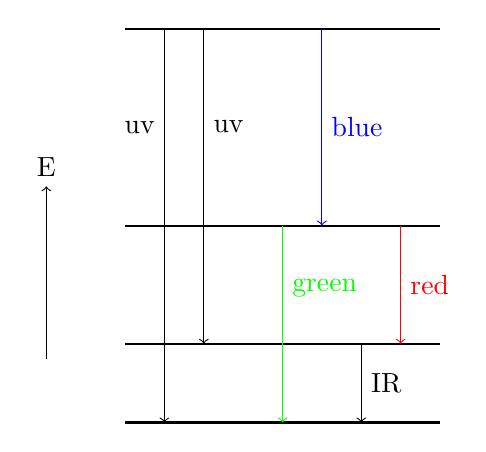
\begin{tikzpicture}

  \draw[thick] (0,5) -- ++(4,0);
  \draw[thick] (0,2.5) -- ++(4,0);
  \draw[thick] (0,1) -- ++(4,0);
  \draw[thick] (0,0) -- ++(4,0);

  \draw[->] (0.5,5) -- (0.5,0) node[pos=0.25, left] {uv};
  \draw[->] (1,5) -- (1,1) node[pos=0.31, right] {uv};

  \draw[->, green] (2,2.5) -- (2,0) node[pos=0.32, right] {green};
  \draw[->, blue] (2.5,5) -- (2.5,2.5) node[pos=0.5, right] {blue};
  \draw[->] (3,1) -- (3,0) node[pos=0.5, right] {IR};
  \draw[->, red] (3.5,2.5) -- (3.5,1) node[pos=0.5, right] {red};

  \draw[->] (-1,0.8) -- (-1,3) node[above] {E};

\end{tikzpicture}
\end{figure}

The lowest-drawn line is the lowest allowed energy level, with energy increasing towards the higher levels.\\
A jump from the highest energy level to the lowest one may generate a photon with too much energy (too short a wavelength) to be visible -- ultraviolet (or even beyond that), while some of the smaller jumps may correspond to visible wavelengths: blue for the more energetic visible ones, green for the mid-range ones, red for the lowest-energy visible jumps. Finally, even smaller jumps may generate invisible frequencies again, such as infrared or beyond.

So when a material emits photons in this manner, we expect to see these very discrete photon wavelengths, and nothing at all in between. Indeed, we can test this. By using a diffraction grating (a concept later introduced in 8.02/8.02x), we can split the light into its constituent colors, in concept not unlike a prism, so that we see the colors laid out in a nice horizontal line, looking very much like pictures of emission and absorption spectra that we have seen earlier, e.g. like this:

%TODO: add image
%\begin{center}
%\includegraphics[scale=0.65]{\pIImages/lec23_hydrogen_emission}
%\end{center}

This is what we would expect to see from a pure-hydrogen source emitting light.

\begin{center}
$\vcenter{\hbox{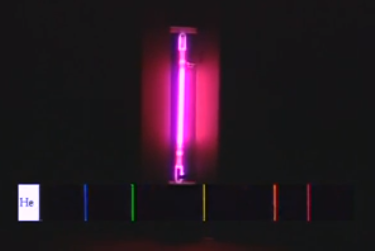
\includegraphics[scale=0.65]{\pIImages/lec34_helium_grating}}}$
$\vcenter{\hbox{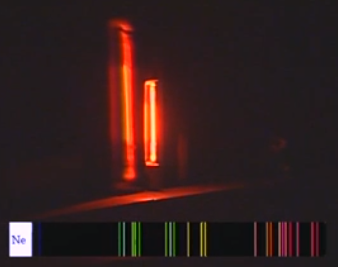
\includegraphics[scale=0.65]{\pIImages/lec34_neon_grating}}}$
\end{center}

Above are two ``simulations'' of the gratings given to the students in lecture, as they could not capture the effect on video. The image on the left is from a helium light source, while that on the right is from a neon light source.

Surprisingly, light also carries momentum! We know that in classical mechanics, $p = m v$, which clearly cannot hold for a photon (if they indeed have nonzero momentum), without some fancy tweaking; the mass of a photon is exactly zero, so $m v = 0$.\\
What we do instead is to use Einstein's mass-energy equivalence, the famous $E = m c^2$:

\begin{equation}
m = \frac{E}{c^2} \Rightarrow p = \frac{E}{c^2} v \Rightarrow p = \frac{E}{c}
\end{equation}

... since $v = c$ for a photon.

We can also find this more directly from the full, less-famous version of the equation:

\begin{equation}
E^2 = (m_0 c^2)^2 + (p c)^2
\end{equation}
where $m_0$ is the rest mass (which I denoted by $m$ above). Since $m_0 = 0$, the equation simplifies down considerably to

\begin{equation}
E = p c
\end{equation}

which is what we found before.

This momentum also gives rise to interesting properties such as radiation pressure/light pressure: shining a light onto something causes a pressure (and therefore a force) due to this momentum transfer! This is used in practice to create spacecraft with ``solar sails'' that use the momentum transfer from reflected light to accelerate. The effect is too tiny to be noticed in daily life, though, considering that visible light has a momentum on the order of perhaps $10^{-27}$ kg m/s per photon. Despite that they come in large numbers, the radiation pressure of for example a regular lamp is negligibly small compared to just about any other force we experience.

\subsection{Wavelength of a particle}

Before quantum mechanics, physicists were divided into two camps: those who thought light to consist of particles, and those who thought it was made of waves.\\
Newton believed that light was made of particles, while Dutch physicist Huygens believed they were waves.\\
In 1801, British scientist Thomas Young showed fairly conclusively that light is a wave, by performing the famous double-slit experiment.\\
You shine a monochromatic light onto two very thin slits in some material (that otherwise blocks light), and project that onto some surface a distance behind.\\
What you see is an interference pattern: there is bright light at the center, then darkness a bit further out, then light again even further out, etc. This can be ``easily'' explained (and is discussed in detail in 8.02/8.02x, and likely even more in detail in 8.03) in terms of light being a wave, as the peaks of the wave cancel out with the valleys when the two arrive in phase, causing darkness; likewise, when two peaks arrive in phase, they add instead of cancel, and the result is a bright area.\\
The two forms of interference are called destructive and constructive interference, respectively.

So it looked like Huygens was right; light is a wave. However, later on, experiments were made that showed quite conclusively that light is made up of particles, perhaps most notably the photoelectric effect observed by Einstein (which won him his only Nobel prize) that required light to arrive in quantized ``packets'' of energy, rather than in a continuous wave. (Einstein didn't discover the effect itself, however.)

Quantum mechanics says the answer to this disagreement is that light acts as \emph{both}, depending on the situation; this concept is known as wave-particle duality.

One of the truly strange things about quantum mechanics is that we can consider \emph{matter particles} to be waves, as well. We now know that finding the wavelength of a photon of some given energy is easy, but what about the wavelength of an electron, or of a baseball?\\
Louis de Broglie suggested that matter can act as waves in this manner. He also specified that the wavelength of such a particle would be

\begin{equation}
\lambda = \frac{h}{p}
\end{equation}

where $p$ is simply the momentum $m v$. We can derive this result ourselves using what we know of the momentum of light.

We know that $E = p c$ and $\displaystyle E = h f = \frac{h c}{\lambda}$; if we put these together, we find

\begin{equation}
p c = \frac{h c}{\lambda} \Rightarrow  p = \frac{h}{\lambda}
\end{equation}

or, equivalently, $\displaystyle \lambda = \frac{h}{p} = \frac{h}{m v}$. This wavelength is called the \emph{de Broglie wavelength}, after him. This derivation assumes that the result is equally valid for matter particles as it is for light, though, which is by no means obvious.

Note that if the momentum is higher, the wavelength is shorter. An electron moving at $10^7$ m/s, and with a rest mass on the order of $10^{-30}$ kg ($9.1\times 10^{-31}$ kg) has a classical momentum of about $\SI{9.1e-24}{kg m/s}$, which translates into a wavelength of about $\lambda = \SI{7.25e-11}{m}$ -- about 73 picometers, several times larger than at atomic nucleus.

A daily life-sized object such a baseball, with a mass of 145 grams, moving at 130 km/h (36.11 m/s) has a momentum of about $5.24$ kg m/s, which gives it a de Broglie wavelength of about $1.3 \times 10^{-34}$ meters -- which is of course ridiculously small. It's far, far below what we could ever measure directly (at a billion billion times smaller than a proton), so this wavelength is meaningless in the macroscopic world. These kinds of quantum effects simply aren't observable at this scale.

\subsection{Heisenberg's uncertainty principle}

In 1926, Austrian physicist Erwin Schr\"odinger formulated the Sch\"odinger equation, which is at the heart of quantum mechanics; it is a wave equation, which describes how a quantum system evolves over time. It unifies these wave and particle behaviors into one set of rules.

We talked earlier about the double-slit experiment and interference of waves. Amazingly, we can do this experiment with particles, too, and get the same end result! This is one of the many extremely nonintuitive results we can find in quantum mechanics.\\
It seems bizarre that e.g. two electrons can be shot through two slits, and then combine and disappear. We really need to think in terms of waves for this to make any sense at all; if the electrons are instead two waves moving through the slits, it does make sense that they can cancel each other out at certain locations.

Let's now look at another bizarre effect in the quantum world. In classical physics, we can measure the momentum and position of an object with any precision that we need, as long as we have the equipment and cleverness. The object has a certain mass, and we can measure its position and momentum at the same time with no problems.

In quantum mechanics, this is not possible. We can measure the position to an arbitrary accuracy, and the momentum to an arbitrary accuracy, but not at the same time! The more exactly we know one, the less exactly we know the other, in this one measurement. This is known as Heisenberg's uncertainty principle.

``The very concept of exact position of an object and its exact momentum, together, have no meaning in nature.''

One way of writing this down mathematically is

\begin{equation}
\Delta p \Delta x \overset{>}{\approx} \frac{\hbar}{2}
\end{equation}

where again $\displaystyle \hbar = \frac{h}{2\pi} \approx 10^{-34}$ joule-seconds.\\
The right-hand side is often written as a factor 2 larger, and I'm not sure which we actually should use. The principle is also often stated in terms of standard deviations. I think we'll have to accept that this is approximate, and take a proper quantum mechanics course for more detail.

Roughly speaking, then, if we know the position to an accuracy $\Delta x$, the momentum is non-determined by an amount

\begin{equation}
\Delta p \overset{>}{\approx} \frac{\hbar}{2 \Delta x}
\end{equation}

The lecture uses twice this ($\hbar$ rather than $\hbar/2$), but there was a caption suggesting that the above values are the ones that \emph{should} have been used in the lecture, i.e. a post-recording correction, so I chose to use their corrected information instead of the one actually shown in the lecture video itself.

The professor uses a story from a book, trying to describe quantum mechanics in an intuitive way (more or less). In this story, we set $\hbar = 1$, instead of about $10^{-34}$. This essentially has the effect of scaling up these quantum effects to a level where we can observe them.\\
So in this world where $\hbar = 1$, a character in the book takes a billiard ball and puts it in a triangle (which is used to align the balls at the start of the game; it can fit exactly 15 such balls in the case of pool).

Assuming the ball stays inside the triangle (which may not be a safe assumption in this crazy quantum world; see quantum tunneling), we have constrained its position to $\Delta x \approx 0.3$ meters. We \emph{know} that it must be somewhere inside the triangle. Via Heisenberg's uncertainty principle, this implies that the ball's momentum is ill-defined to about $1/0.3$ kg m/s (using $\hbar = 1$, and using $\Delta x \Delta p \overset{>}{\approx} \hbar$, as in the lecture), so about 3 kg m/s. If the ball has a mass of 1 kg, the ball's velocity is undetermined to about 3 m/s -- $\Delta p = m \Delta v$. It's moving around like crazy, simply because we constrained its position.

Professor Lewin reads a passage from the book (``the professor'' in what follows refers to a character in the book):

``Look here'', the professor said. ``I'm going to put definite limits on the position of this ball by putting it inside a wooden triangle.''\\
As soon as the ball was placed in the enclosure, the whole inside of the triangle became filled up with the glittering of ivory.\\
''You see'', said the professor, ''I defined the position of the ball to the extent of the dimensions of the triangle. This results in considerable uncertainty in the velocity, and the ball is moving rapidly inside the boundary.\\
''Can't you stop it?'', asks Mr. Tompkins.\\
''No, it is physically impossible. Any body in an enclosed space possess a certain motion. We physicists call it zero point motion. For example, the motion of electrons in any atom.''

So with $\hbar = 1$, the bizarre consequences of the quantum world become more apparent to us, though hardly much easier to grasp.\\
What happens when we perform this experiment in the real world? Well, we perform the same math, but with $\hbar$ being $10^{-34}$ times smaller than above. The effects scales linearly with $\hbar$, so the uncertainty in the ball's velocity is now on the order of $\SI{3e-34}{m/s}$ -- a value so tiny that we could never measure it. In one billion years, the ball would move at most 1/100 of the diameter of a proton. Such distances and velocities are of course completely meaningless to us, and so we again see that these effects are irrelevant in the macroscopic world ``of baseballs and billiards and pots and pans''.

For this reason, it is no problem for us to talk about a billiard ball being exactly at a certain position, and having exactly zero speed. The error is so far beyond measurable that we could never show whether it actually exists or not, so it is completely safe to ignore it and keep working as usual.

Let's now look at an atom, and more specifically the electrons ``orbiting'' it. Say an atom is about $10^{-10}$ meters. An electron is then confined to $\Delta x \approx 10^{-10}$ m. Using the uncertainty principle, we can find that

\begin{align}
m \Delta v \Delta x &\overset{>}{\approx} \hbar\\
\Delta v  &\overset{>}{\approx} \frac{\hbar}{m \Delta x}
\end{align}

(Again, this is using the lecture's possibly incorrect equations and not the ones they later added as corrections via overlaid text, though I'm not sure if either form can be used for accurate calculations.)\\
Using $\Delta x = 10^{-10}$ m and $m \approx 10^{-30}$, we find $\Delta v \overset{>}{\approx} 10^6$ m/s, a third of a percent of the speed of light. So the electron moves simply because it is confined.

\subsection{The single-slit experiment}

The professor then makes a demonstration that can be explained in terms of the uncertainty principle. We shine a laser beam, monochromatic light (i.e. it consists of only one wavelength, as opposed to e.g. white light) onto a thin vertical slit in a material that otherwise blocks light. A distance $L$ away (where $L$ is several meters), we have a wall, that this light pattern is projected upon.

During the experiment, we then shrink the (vertical) slit's width. In doing so, less light will manage to pass through -- that much is clearly unavoidable -- and the laser dot projected on the wall will have its sides ``chopped off'', just as we would predict.\\
However, in doing this, we are constraining $\Delta x$. The thinner the slit is, the better we know the $x$ position of the photons that pass through (if we consider them as photons rather than waves, that is). Because of this, via the uncertainty principle, we lose accuracy in our knowledge of the momentum in the $x$ direction (the direction we are constraining the photons in).
We are not constraining the beam in the $y$ directions, so nothing out of the ordinary will happen in the vertical direction.\\
Horizontally, however, the light begins to \emph{spread out}. The \emph{thinner} the slit becomes, the \emph{wider} the light projection becomes! Simply because we reduce $\Delta x$ and constrain the light's position, the x-component of the momentum is starting to become more and more ill-defined, and some of the light spreads out accordingly.

We can work this out semi-quantitatively. The momentum of each photon is about $10^{-27}$ kg m/s, according to the professor. This indeed corresponds to the wavelength of red light; the laser in the lecture is green, but everything here is an order-of-magnitude approximation, so there's little point in being more precise.\\
Say we start with the slit at 1/10 mm, that is, it can pass though a slit of width $\Delta x \approx 10^{-4}$ meters, constraining its position. That makes the x-component of the momentum ill-defined to about $h/\Delta x \approx 10^{-34} / 10^{-4} = 10^{-30}$ meters. (I'm not sure if $\hbar$ was/should be used here, but it seems it was not; consider this an order-of-magnitude type result either way.)

The total momentum is then the sum of the light's original momentum and this $\Delta p$, so the path changes path according to this vector addition:

\begin{figure}[H]
  \centering
\begin{tikzpicture}

  \node at (0,2) {$\Delta p = \frac{10^{-34}}{10^{-4}} = 10^{-30}$};

  \coordinate (start) at (4,3);
  
  \node[above=2mm] at (start) {$|\Delta x|$};
  \draw[->, red] (start) -- ++(-1,0) node[pos=0.5, above, black] {\rule{4mm}{0.2pt}};
  \draw[->, red] (start) -- ++(1,0) node[below] {$\Delta p$} node[pos=0.5, above, black] {\rule{4mm}{0.2pt}};
  \draw[->, red] (start) -- ++(0,-2) node[right] {$\vec{p}$};
  \draw[->, red] (start) -- ++(-1.5,-3);
  \draw[dotted] (start)++(-1,0) -- ++(0,-2);
  \draw[dotted] (start)++(0,-2) -- ++(-1,0);

\end{tikzpicture}
\end{figure}

We then expect some of the light to shoot off at an angle, but only in the $x$ direction; the light is not constrained at all in the $y$ direction (the slit's height is much greater than the light beam's diameter).

The angle $\theta$ between the original vector and the new one can now be easily calculated. Using trigonometry, $\tan \theta = \Delta p / p$. For small angles, $\tan \theta \approx \sin \theta \approx \theta$, we can consider this simply as $\theta = \Delta p / p$. (The professor did this implicitly.)

For the values we have, with $\Delta x = 1/10$ mm leading to $\Delta p \approx 10^{-30}$ kg m/s, we find $\theta \approx 10^{-3}$ radians. Using the definition of a radian, we can multiply this by the distance $L$ to the screen to get the approximate size at the screen. With $L = 10$ meters, we find $\theta L \approx 1$ cm (in each direction from the center, so a total width of about 2 cm).

However, if we make the slit 10 times smaller, $\Delta p$ grows by 10 times, which causes $\theta$ to grow by 10 times, and therefore $\theta L$ also grows by 10 times. The ``uncertainty'' is now 10 cm in each direction of the center, so the light has spread out way more. This is then demonstrated in the lecture -- which is clearly something that must be \emph{seen}!

The professor then makes it clear that this can be explained without the uncertainty principle -- and was explained to high accuracy even in the 19th century; this demonstration is however entirely consistent with the uncertainty principle.\\
(This experiment is also discussed in further detail in 8.02/8.02x, in the context of interference of light waves and diffraction; there, we also explain the dark bands that appear, that I briefly mentioned in regards to the \emph{double} slit experiment, where they are more prominent and appear in two ways, rather than one way as seen here.)

Modern quantum physics can make some incredibly accurate predictions (I read that in some cases, we can measure quantum phenomena to an accuracy a million times better than that of some astronomical phenomena), however, we cannot predict exactly where each photon is going to end up. Quantum mechanics is, by its very nature, a probability-based theory. We can calculate how the pattern will look after a whole lot of photons have hit the screen, as they are more likely to end up in some places. However, we cannot predict anything at all about what an individual photon will do; as far as we can tell, nature has an intrinsic randomness built into it.

It has been argued that perhaps this behavior is not random; perhaps it would be predictable, only that there are some variables we are not aware of, and that a more complete theory \emph{would} be able to predict all behavior (given all necessary initial conditions). Certain types of these theories seem to have been disproven, and as of yet, there is no proof of these so-called ``hidden variables'' existing, though there is still discussion and research being done in this area, to the best of my understanding. That is, quantum mechanics still appears to be indeterministic: given all possible information about every particle in the universe, you still cannot predict exactly what will happen next, only come up with accurate probabilities.

One more crazy detail in regards to this: it's important to realize that this experiment cannot be adequately explained by photons (particles) interfering with each other. The exact same pattern will build up over time \emph{regardless} of the rate you shoot the photons through. Even if you shoot one photon, wait 5 minutes, shoot the next, etc. the same pattern will emerge over time. The photon must in some way interfere with... itself? This only really makes any kind of sense if we consider waves.

Also, the same experiment can be and has been done with particles, ranging from electrons up to multi-atom structures such as ``buckyballs'' (each of which consists of 60 carbon atoms), and the results are exactly as predicted by quantum mechanics. Photons, electrons or buckyballs -- nature doesn't really care and treats them the same way, it would seem!

\subsection{Some notes on the uncertainty principle}

(This last section is not at all from the lecture, and is (just as the intro section to this lecture) all written by me. That is, you shouldn't take anything in here as hard fact, as I have not studied quantum mechanics to any greater extent than what this course teaches, plus some popular science which often is just as misleading as it is informative.)

A common question (and misconception) is that this uncertainty is a technical limit in our measuring equipment; it is not. It is a physical limit built into nature. I hardly have the expertise (or even basic knowledge) of quantum mechanics to know this myself yet, but many describe the entire notion of perfectly knowing both momentum and position as \emph{meaningless} in quantum mechanics, including that quote in the lecture earlier.

Another common explanation for this uncertainty (one that I've liked myself) is that in order to for example measure the position of an electron, we need to probe it somehow, perhaps using light (sending photons to interact with it). A photon of long wavelength has little energy and thus little momentum, and won't disturb the electron a lot; we get a fairly accurate measurement of its momentum, but since the light wavelength is large, we don't know \emph{exactly} where it is; we only have a fuzzy idea about the position!

If we want to measure the position accurately, we instead need to use light of a shorter wavelength (smaller $\Delta x$), i.e. greater energy (and greater momentum, $p = E/c$ for light). This means we will know where the electron is (was) very accurately, but because we transferred a large amount of momentum to it, we can now not know its momentum exactly.

The above explanation (Heisenberg's microscope) is not technically accurate, though. It is a metaphor, rather than an explanation. In reality, the uncertainty predicted by the uncertainty principle is greater than that in the above experiment.

My current understanding (again, without having actually studied any quantum mechanics -- this is still unlikely to be 100\% correct!) is that the uncertainty arises from the wave nature of matter. That is, the electron doesn't really \emph{have} a perfectly defined position until it is probed; prior to the probing, the electron's position is only a probability distribution. It may be likely to be confined in a small volume, but it is still \emph{possible} for it to be outside it -- even infinitely far away, only with a probability moving closer to 0 the further away you go.

\section{Lecture 35: Professor Lewin's early days at MIT}

I did not take any notes for this lecture. It is as always absolutely worth watching, but it feels pointless to write it down -- professor Lewin is telling \emph{his} story, and I should leave that to \emph{him} to do so! If you want it in text form, his book ``For the Love of Physics'' talks about  these topics and several others!

%%% Local Variables:
%%% TeX-master: "../../main"
%%% End:
